\documentclass[twoside]{book}

% Packages required by doxygen
\usepackage{fixltx2e}
\usepackage{calc}
\usepackage{doxygen}
\usepackage[export]{adjustbox} % also loads graphicx
\usepackage{graphicx}
\usepackage[utf8]{inputenc}
\usepackage{makeidx}
\usepackage{multicol}
\usepackage{multirow}
\PassOptionsToPackage{warn}{textcomp}
\usepackage{textcomp}
\usepackage[nointegrals]{wasysym}
\usepackage[table]{xcolor}

% Font selection
\usepackage[T1]{fontenc}
\usepackage[scaled=.90]{helvet}
\usepackage{courier}
\usepackage{amssymb}
\usepackage{sectsty}
\renewcommand{\familydefault}{\sfdefault}
\allsectionsfont{%
  \fontseries{bc}\selectfont%
  \color{darkgray}%
}
\renewcommand{\DoxyLabelFont}{%
  \fontseries{bc}\selectfont%
  \color{darkgray}%
}
\newcommand{\+}{\discretionary{\mbox{\scriptsize$\hookleftarrow$}}{}{}}

% Page & text layout
\usepackage{geometry}
\geometry{%
  a4paper,%
  top=2.5cm,%
  bottom=2.5cm,%
  left=2.5cm,%
  right=2.5cm%
}
\tolerance=750
\hfuzz=15pt
\hbadness=750
\setlength{\emergencystretch}{15pt}
\setlength{\parindent}{0cm}
\setlength{\parskip}{3ex plus 2ex minus 2ex}
\makeatletter
\renewcommand{\paragraph}{%
  \@startsection{paragraph}{4}{0ex}{-1.0ex}{1.0ex}{%
    \normalfont\normalsize\bfseries\SS@parafont%
  }%
}
\renewcommand{\subparagraph}{%
  \@startsection{subparagraph}{5}{0ex}{-1.0ex}{1.0ex}{%
    \normalfont\normalsize\bfseries\SS@subparafont%
  }%
}
\makeatother

% Headers & footers
\usepackage{fancyhdr}
\pagestyle{fancyplain}
\fancyhead[LE]{\fancyplain{}{\bfseries\thepage}}
\fancyhead[CE]{\fancyplain{}{}}
\fancyhead[RE]{\fancyplain{}{\bfseries\leftmark}}
\fancyhead[LO]{\fancyplain{}{\bfseries\rightmark}}
\fancyhead[CO]{\fancyplain{}{}}
\fancyhead[RO]{\fancyplain{}{\bfseries\thepage}}
\fancyfoot[LE]{\fancyplain{}{}}
\fancyfoot[CE]{\fancyplain{}{}}
\fancyfoot[RE]{\fancyplain{}{\bfseries\scriptsize Generated by Doxygen }}
\fancyfoot[LO]{\fancyplain{}{\bfseries\scriptsize Generated by Doxygen }}
\fancyfoot[CO]{\fancyplain{}{}}
\fancyfoot[RO]{\fancyplain{}{}}
\renewcommand{\footrulewidth}{0.4pt}
\renewcommand{\chaptermark}[1]{%
  \markboth{#1}{}%
}
\renewcommand{\sectionmark}[1]{%
  \markright{\thesection\ #1}%
}

% Indices & bibliography
\usepackage{natbib}
\usepackage[titles]{tocloft}
\setcounter{tocdepth}{3}
\setcounter{secnumdepth}{5}
\makeindex

% Hyperlinks (required, but should be loaded last)
\usepackage{ifpdf}
\ifpdf
  \usepackage[pdftex,pagebackref=true]{hyperref}
\else
  \usepackage[ps2pdf,pagebackref=true]{hyperref}
\fi
\hypersetup{%
  colorlinks=true,%
  linkcolor=blue,%
  citecolor=blue,%
  unicode%
}

% Custom commands
\newcommand{\clearemptydoublepage}{%
  \newpage{\pagestyle{empty}\cleardoublepage}%
}

\usepackage{caption}
\captionsetup{labelsep=space,justification=centering,font={bf},singlelinecheck=off,skip=4pt,position=top}

%===== C O N T E N T S =====

\begin{document}

% Titlepage & ToC
\hypersetup{pageanchor=false,
             bookmarksnumbered=true,
             pdfencoding=unicode
            }
\pagenumbering{alph}
\begin{titlepage}
\vspace*{7cm}
\begin{center}%
{\Large D\+B\+Export \\[1ex]\large 1.\+0.\+0 }\\
\vspace*{1cm}
{\large Generated by Doxygen 1.8.13}\\
\end{center}
\end{titlepage}
\clearemptydoublepage
\pagenumbering{roman}
\tableofcontents
\clearemptydoublepage
\pagenumbering{arabic}
\hypersetup{pageanchor=true}

%--- Begin generated contents ---
\chapter{readme}
\label{md_readme}
\Hypertarget{md_readme}
\input{md_readme}
\chapter{Hierarchical Index}
\section{Class Hierarchy}
This inheritance list is sorted roughly, but not completely, alphabetically\+:\begin{DoxyCompactList}
\item Exception\begin{DoxyCompactList}
\item \contentsline{section}{Export\+Exception}{\pageref{classExportException}}{}
\end{DoxyCompactList}
\item \contentsline{section}{Export\+Model\+Processing}{\pageref{classExportModelProcessing}}{}
\item \contentsline{section}{Message}{\pageref{classMessage}}{}
\end{DoxyCompactList}

\chapter{Class Index}
\section{Class List}
Here are the classes, structs, unions and interfaces with brief descriptions\+:\begin{DoxyCompactList}
\item\contentsline{section}{\hyperlink{classExportException}{Export\+Exception} }{\pageref{classExportException}}{}
\item\contentsline{section}{\hyperlink{classExportModelProcessing}{Export\+Model\+Processing} }{\pageref{classExportModelProcessing}}{}
\item\contentsline{section}{\hyperlink{classMessage}{Message} }{\pageref{classMessage}}{}
\end{DoxyCompactList}

\chapter{Class Documentation}
\hypertarget{classExportException}{}\section{Export\+Exception Class Reference}
\label{classExportException}\index{Export\+Exception@{Export\+Exception}}


Inheritance diagram for Export\+Exception\+:
\nopagebreak
\begin{figure}[H]
\begin{center}
\leavevmode
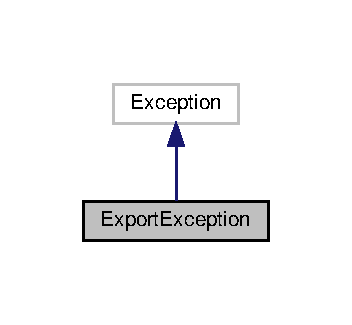
\includegraphics[width=169pt]{classExportException__inherit__graph}
\end{center}
\end{figure}


Collaboration diagram for Export\+Exception\+:
\nopagebreak
\begin{figure}[H]
\begin{center}
\leavevmode
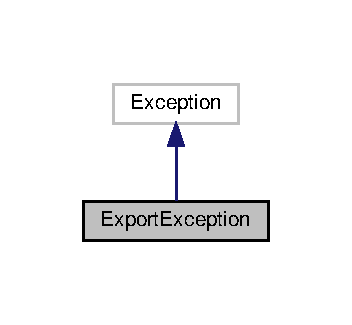
\includegraphics[width=169pt]{classExportException__coll__graph}
\end{center}
\end{figure}


The documentation for this class was generated from the following file\+:\begin{DoxyCompactItemize}
\item 
exportmodel.\+class.\+php\end{DoxyCompactItemize}

\hypertarget{classExportModelProcessing}{}\section{Export\+Model\+Processing Class Reference}
\label{classExportModelProcessing}\index{Export\+Model\+Processing@{Export\+Model\+Processing}}
\subsection*{Public Member Functions}
\begin{DoxyCompactItemize}
\item 
\hyperlink{classExportModelProcessing_a5f3544bdd5de2c528d301db24751a90a}{\+\_\+\+\_\+construct} (P\+DO \$db)
\item 
\mbox{\Hypertarget{classExportModelProcessing_a43f822b0753caf336b74abe8e60f14b3}\label{classExportModelProcessing_a43f822b0753caf336b74abe8e60f14b3}} 
{\bfseries set\+Default\+Path} (string \$path)
\item 
\hyperlink{classExportModelProcessing_ab74a02a40ccfff57494986e1c038cad5}{init\+Model} (array \$model)
\item 
\hyperlink{classExportModelProcessing_a2e0ab00ea8525229c72da1abda3d3043}{init\+Structure} (array \$structure=array())
\item 
\hyperlink{classExportModelProcessing_a2c083b18ab22fc95db1939ccf14c9a46}{generate\+Structure} (array \$model=array())
\item 
\hyperlink{classExportModelProcessing_ae31ea6c13d62aebabcdd2a6ff904474b}{get\+Description\+From\+Table} (string \$tablename, string \$schemaname=\char`\"{}\char`\"{})
\item 
\hyperlink{classExportModelProcessing_a1bc41fccfbce6de5b4e167eb9937f488}{get\+Fields\+From\+Table} (string \$tablename, string \$schemaname=\char`\"{}\char`\"{})
\item 
\hyperlink{classExportModelProcessing_a55bf879da8bb3b010e36939195ff7756}{generate\+Create\+Sql} (array \$structure=array())
\item 
\hyperlink{classExportModelProcessing_ae891c1f59aee9f32d1de48d4e88bec19}{get\+Primary\+Key} (array \$table)
\item 
\hyperlink{classExportModelProcessing_a2f3b9bd68cbcef66ed9acd888ceb65a2}{generate\+Sql\+Relation} (string \$parent\+Table, string \$parent\+Key, string \$child\+Table, string \$child\+Foreign\+Key)
\item 
\hyperlink{classExportModelProcessing_adfa4dd7271ec720245cb2f6845b983cc}{generate\+Sql\+For\+Table} (string \$table\+Name, array \$table)
\item 
\hyperlink{classExportModelProcessing_a92d950555aa256e6ef6ceb0a976e83e5}{get\+List\+Primary\+Tables} ()
\item 
\hyperlink{classExportModelProcessing_a66a3f33cd27c03c19b07f4074bab3cd8}{generate\+List\+Columns} (string \$table\+Name)
\item 
\hyperlink{classExportModelProcessing_a048a271e644dfa50549826dce12737bd}{get\+Specific\+Fields} (array \$attributes, string \$field\+Type)
\item 
\hyperlink{classExportModelProcessing_a788bed37275c67ecefa4b249a0f8910b}{get\+Table\+Content} (string \$table\+Alias, array \$keys=array(), int \$parent\+Key=0)
\item 
\hyperlink{classExportModelProcessing_a35cfd1e3beb5e7dc9a47d8cc262b2c93}{get\+Blob\+Reference} (string \$table\+Name, string \$key\+Name, int \$id, string \$field\+Name)
\item 
\hyperlink{classExportModelProcessing_ab64c8d4090ae54eb8b3a55853810b014}{import\+Data} (array \$data)
\item 
\hyperlink{classExportModelProcessing_a713672fd704e7044319586d7bda6e712}{import\+Data\+Table} (string \$table\+Alias, array \$data, int \$parent\+Key=0, array \$set\+Values=array(), \$delete\+Before\+Insert=false)
\item 
\hyperlink{classExportModelProcessing_a2038baafaded8f112fecf777792a3204}{write\+Data} (string \$table\+Alias, array \$data)
\end{DoxyCompactItemize}
\subsection*{Public Attributes}
\begin{DoxyCompactItemize}
\item 
\mbox{\Hypertarget{classExportModelProcessing_a897c1e7cad4956ffd342ea962f687f21}\label{classExportModelProcessing_a897c1e7cad4956ffd342ea962f687f21}} 
{\bfseries \$mode\+Debug} = false
\item 
\mbox{\Hypertarget{classExportModelProcessing_a3a144b354537209ed78f6cf4428bc5cb}\label{classExportModelProcessing_a3a144b354537209ed78f6cf4428bc5cb}} 
{\bfseries \$structure} = array()
\item 
\mbox{\Hypertarget{classExportModelProcessing_a3574016a0a223da71e37af1a73b5b1b2}\label{classExportModelProcessing_a3574016a0a223da71e37af1a73b5b1b2}} 
{\bfseries \$quote} = \textquotesingle{}\char`\"{}\textquotesingle{}
\item 
\mbox{\Hypertarget{classExportModelProcessing_a67d1483753c4fa6b0543aceaf3664e51}\label{classExportModelProcessing_a67d1483753c4fa6b0543aceaf3664e51}} 
{\bfseries \$binary\+Folder} = \char`\"{}binary\char`\"{}
\end{DoxyCompactItemize}


\subsection{Constructor \& Destructor Documentation}
\mbox{\Hypertarget{classExportModelProcessing_a5f3544bdd5de2c528d301db24751a90a}\label{classExportModelProcessing_a5f3544bdd5de2c528d301db24751a90a}} 
\index{Export\+Model\+Processing@{Export\+Model\+Processing}!\+\_\+\+\_\+construct@{\+\_\+\+\_\+construct}}
\index{\+\_\+\+\_\+construct@{\+\_\+\+\_\+construct}!Export\+Model\+Processing@{Export\+Model\+Processing}}
\subsubsection{\texorpdfstring{\+\_\+\+\_\+construct()}{\_\_construct()}}
{\footnotesize\ttfamily Export\+Model\+Processing\+::\+\_\+\+\_\+construct (\begin{DoxyParamCaption}\item[{P\+DO}]{\$db }\end{DoxyParamCaption})}

Constructor


\begin{DoxyParams}[1]{Parameters}
P\+DO & {\em \$bdd,} & database connection object \\
\hline
\end{DoxyParams}


\subsection{Member Function Documentation}
\mbox{\Hypertarget{classExportModelProcessing_a55bf879da8bb3b010e36939195ff7756}\label{classExportModelProcessing_a55bf879da8bb3b010e36939195ff7756}} 
\index{Export\+Model\+Processing@{Export\+Model\+Processing}!generate\+Create\+Sql@{generate\+Create\+Sql}}
\index{generate\+Create\+Sql@{generate\+Create\+Sql}!Export\+Model\+Processing@{Export\+Model\+Processing}}
\subsubsection{\texorpdfstring{generate\+Create\+Sql()}{generateCreateSql()}}
{\footnotesize\ttfamily Export\+Model\+Processing\+::generate\+Create\+Sql (\begin{DoxyParamCaption}\item[{array}]{\$structure = {\ttfamily array()} }\end{DoxyParamCaption})}

Generate the sql script to create the tables in the database


\begin{DoxyParams}[1]{Parameters}
array & {\em \$structure} & \\
\hline
\end{DoxyParams}
\begin{DoxyReturn}{Returns}
string 
\end{DoxyReturn}
Creation of tables

Creation of relations\mbox{\Hypertarget{classExportModelProcessing_a66a3f33cd27c03c19b07f4074bab3cd8}\label{classExportModelProcessing_a66a3f33cd27c03c19b07f4074bab3cd8}} 
\index{Export\+Model\+Processing@{Export\+Model\+Processing}!generate\+List\+Columns@{generate\+List\+Columns}}
\index{generate\+List\+Columns@{generate\+List\+Columns}!Export\+Model\+Processing@{Export\+Model\+Processing}}
\subsubsection{\texorpdfstring{generate\+List\+Columns()}{generateListColumns()}}
{\footnotesize\ttfamily Export\+Model\+Processing\+::generate\+List\+Columns (\begin{DoxyParamCaption}\item[{string}]{\$table\+Name }\end{DoxyParamCaption})}

Prepare the list of columns for sql clause


\begin{DoxyParams}[1]{Parameters}
string & {\em \$table\+Name} & \\
\hline
\end{DoxyParams}
\begin{DoxyReturn}{Returns}
string 
\end{DoxyReturn}
\mbox{\Hypertarget{classExportModelProcessing_adfa4dd7271ec720245cb2f6845b983cc}\label{classExportModelProcessing_adfa4dd7271ec720245cb2f6845b983cc}} 
\index{Export\+Model\+Processing@{Export\+Model\+Processing}!generate\+Sql\+For\+Table@{generate\+Sql\+For\+Table}}
\index{generate\+Sql\+For\+Table@{generate\+Sql\+For\+Table}!Export\+Model\+Processing@{Export\+Model\+Processing}}
\subsubsection{\texorpdfstring{generate\+Sql\+For\+Table()}{generateSqlForTable()}}
{\footnotesize\ttfamily Export\+Model\+Processing\+::generate\+Sql\+For\+Table (\begin{DoxyParamCaption}\item[{string}]{\$table\+Name,  }\item[{array}]{\$table }\end{DoxyParamCaption})}

Generate the sql code for create a table in the database


\begin{DoxyParams}[1]{Parameters}
string & {\em \$table\+Name} & \\
\hline
array & {\em \$table} & \\
\hline
\end{DoxyParams}
\begin{DoxyReturn}{Returns}
string 
\end{DoxyReturn}
Add the comment of the table

Add the comment on the column

Add the primary key\mbox{\Hypertarget{classExportModelProcessing_a2f3b9bd68cbcef66ed9acd888ceb65a2}\label{classExportModelProcessing_a2f3b9bd68cbcef66ed9acd888ceb65a2}} 
\index{Export\+Model\+Processing@{Export\+Model\+Processing}!generate\+Sql\+Relation@{generate\+Sql\+Relation}}
\index{generate\+Sql\+Relation@{generate\+Sql\+Relation}!Export\+Model\+Processing@{Export\+Model\+Processing}}
\subsubsection{\texorpdfstring{generate\+Sql\+Relation()}{generateSqlRelation()}}
{\footnotesize\ttfamily Export\+Model\+Processing\+::generate\+Sql\+Relation (\begin{DoxyParamCaption}\item[{string}]{\$parent\+Table,  }\item[{string}]{\$parent\+Key,  }\item[{string}]{\$child\+Table,  }\item[{string}]{\$child\+Foreign\+Key }\end{DoxyParamCaption})}

Generate the sql script for create a relationship between 2 tables


\begin{DoxyParams}[1]{Parameters}
string & {\em \$parent\+Table} & \\
\hline
string & {\em \$parent\+Key} & \\
\hline
string & {\em \$child\+Table} & \\
\hline
string & {\em \$child\+Foreign\+Key} & \\
\hline
\end{DoxyParams}
\begin{DoxyReturn}{Returns}
string 
\end{DoxyReturn}
\mbox{\Hypertarget{classExportModelProcessing_a2c083b18ab22fc95db1939ccf14c9a46}\label{classExportModelProcessing_a2c083b18ab22fc95db1939ccf14c9a46}} 
\index{Export\+Model\+Processing@{Export\+Model\+Processing}!generate\+Structure@{generate\+Structure}}
\index{generate\+Structure@{generate\+Structure}!Export\+Model\+Processing@{Export\+Model\+Processing}}
\subsubsection{\texorpdfstring{generate\+Structure()}{generateStructure()}}
{\footnotesize\ttfamily Export\+Model\+Processing\+::generate\+Structure (\begin{DoxyParamCaption}\item[{array}]{\$model = {\ttfamily array()} }\end{DoxyParamCaption})}

Generate the structure of database for all tables in the model


\begin{DoxyParams}[1]{Parameters}
array & {\em \$model} & \\
\hline
\end{DoxyParams}
\begin{DoxyReturn}{Returns}
array 
\end{DoxyReturn}
Get specific fields

Add the children

Add the parents (parameters tables, table nn)

Add the second n-\/n part\mbox{\Hypertarget{classExportModelProcessing_a35cfd1e3beb5e7dc9a47d8cc262b2c93}\label{classExportModelProcessing_a35cfd1e3beb5e7dc9a47d8cc262b2c93}} 
\index{Export\+Model\+Processing@{Export\+Model\+Processing}!get\+Blob\+Reference@{get\+Blob\+Reference}}
\index{get\+Blob\+Reference@{get\+Blob\+Reference}!Export\+Model\+Processing@{Export\+Model\+Processing}}
\subsubsection{\texorpdfstring{get\+Blob\+Reference()}{getBlobReference()}}
{\footnotesize\ttfamily Export\+Model\+Processing\+::get\+Blob\+Reference (\begin{DoxyParamCaption}\item[{string}]{\$table\+Name,  }\item[{string}]{\$key\+Name,  }\item[{int}]{\$id,  }\item[{string}]{\$field\+Name }\end{DoxyParamCaption})}

Read a binary object in the database and returns the resource file


\begin{DoxyParams}[1]{Parameters}
string & {\em \$table\+Name} & \\
\hline
string & {\em \$key\+Name} & \\
\hline
integer & {\em \$id} & \\
\hline
string & {\em \$field\+Name} & \\
\hline
\end{DoxyParams}
\begin{DoxyReturn}{Returns}
resource$\vert$null 
\end{DoxyReturn}
\mbox{\Hypertarget{classExportModelProcessing_ae31ea6c13d62aebabcdd2a6ff904474b}\label{classExportModelProcessing_ae31ea6c13d62aebabcdd2a6ff904474b}} 
\index{Export\+Model\+Processing@{Export\+Model\+Processing}!get\+Description\+From\+Table@{get\+Description\+From\+Table}}
\index{get\+Description\+From\+Table@{get\+Description\+From\+Table}!Export\+Model\+Processing@{Export\+Model\+Processing}}
\subsubsection{\texorpdfstring{get\+Description\+From\+Table()}{getDescriptionFromTable()}}
{\footnotesize\ttfamily Export\+Model\+Processing\+::get\+Description\+From\+Table (\begin{DoxyParamCaption}\item[{string}]{\$tablename,  }\item[{string}]{\$schemaname = {\ttfamily \char`\"{}\char`\"{}} }\end{DoxyParamCaption})}

Get the comment associated to a table


\begin{DoxyParams}[1]{Parameters}
string & {\em \$tablename} & \\
\hline
string & {\em \$schemaname} & \\
\hline
\end{DoxyParams}
\begin{DoxyReturn}{Returns}
string 
\end{DoxyReturn}
\mbox{\Hypertarget{classExportModelProcessing_a1bc41fccfbce6de5b4e167eb9937f488}\label{classExportModelProcessing_a1bc41fccfbce6de5b4e167eb9937f488}} 
\index{Export\+Model\+Processing@{Export\+Model\+Processing}!get\+Fields\+From\+Table@{get\+Fields\+From\+Table}}
\index{get\+Fields\+From\+Table@{get\+Fields\+From\+Table}!Export\+Model\+Processing@{Export\+Model\+Processing}}
\subsubsection{\texorpdfstring{get\+Fields\+From\+Table()}{getFieldsFromTable()}}
{\footnotesize\ttfamily Export\+Model\+Processing\+::get\+Fields\+From\+Table (\begin{DoxyParamCaption}\item[{string}]{\$tablename,  }\item[{string}]{\$schemaname = {\ttfamily \char`\"{}\char`\"{}} }\end{DoxyParamCaption})}

Get the list of columns of the table


\begin{DoxyParams}[1]{Parameters}
string & {\em \$tablename} & \\
\hline
\end{DoxyParams}
\begin{DoxyReturn}{Returns}
array$\vert$null 
\end{DoxyReturn}
translate sequence field to serial\mbox{\Hypertarget{classExportModelProcessing_a92d950555aa256e6ef6ceb0a976e83e5}\label{classExportModelProcessing_a92d950555aa256e6ef6ceb0a976e83e5}} 
\index{Export\+Model\+Processing@{Export\+Model\+Processing}!get\+List\+Primary\+Tables@{get\+List\+Primary\+Tables}}
\index{get\+List\+Primary\+Tables@{get\+List\+Primary\+Tables}!Export\+Model\+Processing@{Export\+Model\+Processing}}
\subsubsection{\texorpdfstring{get\+List\+Primary\+Tables()}{getListPrimaryTables()}}
{\footnotesize\ttfamily Export\+Model\+Processing\+::get\+List\+Primary\+Tables (\begin{DoxyParamCaption}{ }\end{DoxyParamCaption})}

Get the list of the tables which are not children

\begin{DoxyReturn}{Returns}
array 
\end{DoxyReturn}
\mbox{\Hypertarget{classExportModelProcessing_ae891c1f59aee9f32d1de48d4e88bec19}\label{classExportModelProcessing_ae891c1f59aee9f32d1de48d4e88bec19}} 
\index{Export\+Model\+Processing@{Export\+Model\+Processing}!get\+Primary\+Key@{get\+Primary\+Key}}
\index{get\+Primary\+Key@{get\+Primary\+Key}!Export\+Model\+Processing@{Export\+Model\+Processing}}
\subsubsection{\texorpdfstring{get\+Primary\+Key()}{getPrimaryKey()}}
{\footnotesize\ttfamily Export\+Model\+Processing\+::get\+Primary\+Key (\begin{DoxyParamCaption}\item[{array}]{\$table }\end{DoxyParamCaption})}

Get the primary key of a table from structure


\begin{DoxyParams}[1]{Parameters}
array & {\em \$table} & \\
\hline
\end{DoxyParams}
\begin{DoxyReturn}{Returns}
string 
\end{DoxyReturn}
\mbox{\Hypertarget{classExportModelProcessing_a048a271e644dfa50549826dce12737bd}\label{classExportModelProcessing_a048a271e644dfa50549826dce12737bd}} 
\index{Export\+Model\+Processing@{Export\+Model\+Processing}!get\+Specific\+Fields@{get\+Specific\+Fields}}
\index{get\+Specific\+Fields@{get\+Specific\+Fields}!Export\+Model\+Processing@{Export\+Model\+Processing}}
\subsubsection{\texorpdfstring{get\+Specific\+Fields()}{getSpecificFields()}}
{\footnotesize\ttfamily Export\+Model\+Processing\+::get\+Specific\+Fields (\begin{DoxyParamCaption}\item[{array}]{\$attributes,  }\item[{string}]{\$field\+Type }\end{DoxyParamCaption})}

Get the list of specific fields for a table


\begin{DoxyParams}[1]{Parameters}
array & {\em \$table\+Name} & \\
\hline
string & {\em \$field\+Type} & \\
\hline
\end{DoxyParams}
\begin{DoxyReturn}{Returns}
array 
\end{DoxyReturn}
\mbox{\Hypertarget{classExportModelProcessing_a788bed37275c67ecefa4b249a0f8910b}\label{classExportModelProcessing_a788bed37275c67ecefa4b249a0f8910b}} 
\index{Export\+Model\+Processing@{Export\+Model\+Processing}!get\+Table\+Content@{get\+Table\+Content}}
\index{get\+Table\+Content@{get\+Table\+Content}!Export\+Model\+Processing@{Export\+Model\+Processing}}
\subsubsection{\texorpdfstring{get\+Table\+Content()}{getTableContent()}}
{\footnotesize\ttfamily Export\+Model\+Processing\+::get\+Table\+Content (\begin{DoxyParamCaption}\item[{string}]{\$table\+Alias,  }\item[{array}]{\$keys = {\ttfamily array()},  }\item[{int}]{\$parent\+Key = {\ttfamily 0} }\end{DoxyParamCaption})}

Get the content of a table


\begin{DoxyParams}[1]{Parameters}
string & {\em \$table\+Name,} & alias of the table \\
\hline
array & {\em \$keys,} & list of the keys to extract \\
\hline
integer & {\em \$parent\+Key,} & value of the technical\+Key of the parent (foreign key) \\
\hline
\end{DoxyParams}
\begin{DoxyReturn}{Returns}
array 
\end{DoxyReturn}
Search by parent

export the binary data in files

Verifiy if a business key is defined

Verify if binary folder exists

get the description of the secondary table

Search the data from the children

Search the parameters

Get the record associated with the current record\mbox{\Hypertarget{classExportModelProcessing_ab64c8d4090ae54eb8b3a55853810b014}\label{classExportModelProcessing_ab64c8d4090ae54eb8b3a55853810b014}} 
\index{Export\+Model\+Processing@{Export\+Model\+Processing}!import\+Data@{import\+Data}}
\index{import\+Data@{import\+Data}!Export\+Model\+Processing@{Export\+Model\+Processing}}
\subsubsection{\texorpdfstring{import\+Data()}{importData()}}
{\footnotesize\ttfamily Export\+Model\+Processing\+::import\+Data (\begin{DoxyParamCaption}\item[{array}]{\$data }\end{DoxyParamCaption})}

Import data into the database


\begin{DoxyParams}[1]{Parameters}
array & {\em \$data} & \\
\hline
\end{DoxyParams}
\begin{DoxyReturn}{Returns}
void 
\end{DoxyReturn}
\mbox{\Hypertarget{classExportModelProcessing_a713672fd704e7044319586d7bda6e712}\label{classExportModelProcessing_a713672fd704e7044319586d7bda6e712}} 
\index{Export\+Model\+Processing@{Export\+Model\+Processing}!import\+Data\+Table@{import\+Data\+Table}}
\index{import\+Data\+Table@{import\+Data\+Table}!Export\+Model\+Processing@{Export\+Model\+Processing}}
\subsubsection{\texorpdfstring{import\+Data\+Table()}{importDataTable()}}
{\footnotesize\ttfamily Export\+Model\+Processing\+::import\+Data\+Table (\begin{DoxyParamCaption}\item[{string}]{\$table\+Alias,  }\item[{array}]{\$data,  }\item[{int}]{\$parent\+Key = {\ttfamily 0},  }\item[{array}]{\$set\+Values = {\ttfamily array()},  }\item[{}]{\$delete\+Before\+Insert = {\ttfamily false} }\end{DoxyParamCaption})}

Import data from a table


\begin{DoxyParams}[1]{Parameters}
string & {\em \$table\+Name,} & name of the table \\
\hline
array & {\em \$data,} & all data to be recorded \\
\hline
integer & {\em \$parent\+Key,} & key of the parent from the table \\
\hline
array & {\em \$set\+Values,} & list of values to insert into each row. Used for set a parent key \\
\hline
bool & {\em \$delete\+Before\+Insert,} & delete all records linked to the parent before insert new records \\
\hline
\end{DoxyParams}
\begin{DoxyReturn}{Returns}
void 
\end{DoxyReturn}
prepare sql request for searching key

delete pre-\/existent rows

search for preexisting record

Search id of secondary table

write the secondary parent

Get the real values for parameters

Search the id from the parameter

write the parameter

Search the name of the attribute corresponding in the row

Set values

Write data

Record the children\mbox{\Hypertarget{classExportModelProcessing_ab74a02a40ccfff57494986e1c038cad5}\label{classExportModelProcessing_ab74a02a40ccfff57494986e1c038cad5}} 
\index{Export\+Model\+Processing@{Export\+Model\+Processing}!init\+Model@{init\+Model}}
\index{init\+Model@{init\+Model}!Export\+Model\+Processing@{Export\+Model\+Processing}}
\subsubsection{\texorpdfstring{init\+Model()}{initModel()}}
{\footnotesize\ttfamily Export\+Model\+Processing\+::init\+Model (\begin{DoxyParamCaption}\item[{array}]{\$model }\end{DoxyParamCaption})}

Set the used model


\begin{DoxyParams}[1]{Parameters}
array & {\em \$model,} & J\+S\+ON field contents the description of the tables \\
\hline
\end{DoxyParams}
\begin{DoxyReturn}{Returns}
void 
\end{DoxyReturn}
Generate the model with table\+Name as identifier

Set the table\+Alias if not defined\mbox{\Hypertarget{classExportModelProcessing_a2e0ab00ea8525229c72da1abda3d3043}\label{classExportModelProcessing_a2e0ab00ea8525229c72da1abda3d3043}} 
\index{Export\+Model\+Processing@{Export\+Model\+Processing}!init\+Structure@{init\+Structure}}
\index{init\+Structure@{init\+Structure}!Export\+Model\+Processing@{Export\+Model\+Processing}}
\subsubsection{\texorpdfstring{init\+Structure()}{initStructure()}}
{\footnotesize\ttfamily Export\+Model\+Processing\+::init\+Structure (\begin{DoxyParamCaption}\item[{array}]{\$structure = {\ttfamily array()} }\end{DoxyParamCaption})}

Load the structure of the database


\begin{DoxyParams}[1]{Parameters}
array & {\em \$structure} & \\
\hline
\end{DoxyParams}
\begin{DoxyReturn}{Returns}
void 
\end{DoxyReturn}
\mbox{\Hypertarget{classExportModelProcessing_a2038baafaded8f112fecf777792a3204}\label{classExportModelProcessing_a2038baafaded8f112fecf777792a3204}} 
\index{Export\+Model\+Processing@{Export\+Model\+Processing}!write\+Data@{write\+Data}}
\index{write\+Data@{write\+Data}!Export\+Model\+Processing@{Export\+Model\+Processing}}
\subsubsection{\texorpdfstring{write\+Data()}{writeData()}}
{\footnotesize\ttfamily Export\+Model\+Processing\+::write\+Data (\begin{DoxyParamCaption}\item[{string}]{\$table\+Alias,  }\item[{array}]{\$data }\end{DoxyParamCaption})}

insert or update a record


\begin{DoxyParams}[1]{Parameters}
string & {\em \$table\+Name,} & name of the table \\
\hline
array & {\em \$data,} & data of the record \\
\hline
\end{DoxyParams}
\begin{DoxyReturn}{Returns}
int$\vert$null\+: technical key generated or updated 
\end{DoxyReturn}
Search if the record exists

update

insert

Get the binary data

The documentation for this class was generated from the following file\+:\begin{DoxyCompactItemize}
\item 
exportmodel.\+class.\+php\end{DoxyCompactItemize}

\hypertarget{classMessage}{}\section{Message Class Reference}
\label{classMessage}\index{Message@{Message}}
\subsection*{Public Member Functions}
\begin{DoxyCompactItemize}
\item 
\mbox{\Hypertarget{classMessage_af63a9fa2f7f10cb76bd52a01ce8a8559}\label{classMessage_af63a9fa2f7f10cb76bd52a01ce8a8559}} 
{\bfseries \+\_\+\+\_\+construct} (\$display\+Syslog=false)
\item 
\mbox{\Hypertarget{classMessage_a115ff814c66f0e1f187bd737d8a8722c}\label{classMessage_a115ff814c66f0e1f187bd737d8a8722c}} 
{\bfseries set} (\$value, \$is\+\_\+error=false)
\item 
\mbox{\Hypertarget{classMessage_aca32b4947d0e54e39c22d359f6ae4a33}\label{classMessage_aca32b4947d0e54e39c22d359f6ae4a33}} 
{\bfseries set\+Syslog} (\$value)
\item 
\hyperlink{classMessage_a895ffe0bb3e37dab6e7f5b53751e4fb7}{get} ()
\item 
\hyperlink{classMessage_a09832b55a8b16c93af3a503f96d1c8d4}{get\+As\+Html} ()
\end{DoxyCompactItemize}
\subsection*{Public Attributes}
\begin{DoxyCompactItemize}
\item 
\mbox{\Hypertarget{classMessage_a265612c70c7f8fd3e3e7a789528a97eb}\label{classMessage_a265612c70c7f8fd3e3e7a789528a97eb}} 
{\bfseries \$is\+\_\+error} = false
\end{DoxyCompactItemize}


\subsection{Member Function Documentation}
\mbox{\Hypertarget{classMessage_a895ffe0bb3e37dab6e7f5b53751e4fb7}\label{classMessage_a895ffe0bb3e37dab6e7f5b53751e4fb7}} 
\index{Message@{Message}!get@{get}}
\index{get@{get}!Message@{Message}}
\subsubsection{\texorpdfstring{get()}{get()}}
{\footnotesize\ttfamily Message\+::get (\begin{DoxyParamCaption}{ }\end{DoxyParamCaption})}

Retourne le tableau brut \mbox{\Hypertarget{classMessage_a09832b55a8b16c93af3a503f96d1c8d4}\label{classMessage_a09832b55a8b16c93af3a503f96d1c8d4}} 
\index{Message@{Message}!get\+As\+Html@{get\+As\+Html}}
\index{get\+As\+Html@{get\+As\+Html}!Message@{Message}}
\subsubsection{\texorpdfstring{get\+As\+Html()}{getAsHtml()}}
{\footnotesize\ttfamily Message\+::get\+As\+Html (\begin{DoxyParamCaption}{ }\end{DoxyParamCaption})}

Retourne le tableau formate avec saut de ligne entre chaque message

\begin{DoxyReturn}{Returns}
string 
\end{DoxyReturn}


The documentation for this class was generated from the following file\+:\begin{DoxyCompactItemize}
\item 
message.\+php\end{DoxyCompactItemize}

%--- End generated contents ---

% Index
\backmatter
\newpage
\phantomsection
\clearemptydoublepage
\addcontentsline{toc}{chapter}{Index}
\printindex

\end{document}
